\usepackage{nag} % 检测宏包是否过期

%
%原来我把学号打错了,道个歉。。









%%%%%%%%%%%%%%%%%%
% 标题格式
%%%%%%%%%%%%%%%%%%
\ctexset{
    contentsname = {目\quad 录},
    %appendix/name = {附\quad 录}, % NK似乎没打算让我们有多个附录
    proofname = {\indent \normalfont \heiti 证},
    bibname = {参考文献},
    %
    section/name = {,、},
    section/number = \chinese{section},
    section/aftername = \hspace{0pt},
    section/format += \zihao{-3},
    %
    subsection/name =  {(,)},
    subsection/number = \chinese{subsection},
    subsection/aftername = \hspace{0pt},
    subsection/format += \zihao{4},
    %
    subsubsection/number = \arabic{subsubsection},
    subsubsection/name = {,.},
    %subsubsection/aftername = \hspace{0pt},
    subsubsection/format += \zihao{-4}
}

\pagestyle{plain} % 取消页眉




%%%%%%%%%%%%%%%%%%
% 数学公式、定理环境
%%%%%%%%%%%%%%%%%%
\usepackage{amsmath, amsfonts, amsthm}
\usepackage{amssymb, latexsym}
\usepackage{bm} % 数学字体
\usepackage{bbm}

%\newtheorem*{proof}{\hspace{2em}证明} % ams宏包自带proof
\theoremstyle{plain}
\newtheorem{theorem}{定理}
\newtheorem{corollary}{推论}
\newtheorem*{lemma}{引理}
\newtheorem{proposition}{命题}
\newtheorem{assumption}{假设}

\theoremstyle{definition}
\newtheorem{definition}{定义}
\newtheorem{example}{例}

\theoremstyle{remark}
\newtheorem{remark}{\indent \normalfont \heiti 注}

\renewcommand\qedsymbol{\ensuremath{\blacksquare}}
%\numberwithin{equation}{section} % 公式根据 section 编号
%\renewcommand{\proofname}{\indent \normalfont \heiti 证} % 已经在ctex中设置了





%%%%%%%%%%%%%%%%%%
% 图表
%%%%%%%%%%%%%%%%%%
\usepackage[inline]{enumitem} % 可以自定义列表编号,提供行内列表
\usepackage[labelsep=quad]{caption} % 设置表格标题间距 用space太窄 quad太宽 MD
\captionsetup[table]{skip=10pt}
%\captionsetup[lstlisting]{name=代码}
\usepackage{subcaption}
\usepackage{booktabs} % 三线表
\usepackage{diagbox} % 对表头用斜线分割
\usepackage{multirow} % 纵向合并单元格
%\usepackage{tabu} % 该包已经停止维护
%\usepackage{tabularx} % 为与hyperref兼容,在200行导入
\usepackage{longtable} % 跨页表格
\usepackage{multirow} % 表格跨行单元格
\usepackage{graphicx} % 插入图片
\usepackage{float}




%%%%%%%%%%%%%%%%%%
% 目录
%%%%%%%%%%%%%%%%%%
\usepackage[nottoc,numbib]{tocbibind} % 参考文献出现在目录中
\usepackage[subfigure, titles]{tocloft} % 目录 加点 但会改变 “目录”二字 % 根据文档,这两个option都要加
\renewcommand{\cftsecleader}{\cftdotfill{\cftdotsep}}
\setlength\cftsubsubsecnumwidth{1.5em} % 修复目录中subsubsection过深的bug % 调整了package顺序后,bug消失了……




%%%%%%%%%%%%%%%%%%
% 脚注
%%%%%%%%%%%%%%%%%%
\usepackage{pifont}  % footnote格式
\renewcommand\thefootnote{\ding{\numexpr171+\value{footnote}}}
\usepackage[perpage]{footmisc} % 脚注每页从1开始编号
%\renewcommand{\footnotesize}{\zihao{-5}} % 默认就是小五


%%%%%%%%%%%%%%%%%%
% 字体
%%%%%%%%%%%%%%%%%%
\usepackage[T1]{fontenc}  % 使用Times New Roman 字体
\usepackage{mathptmx}% https://liam.page/2017/01/10/Times-New-Roman-and-LaTeX/
%\usepackage{newtxtext, newtxmath} % 另一种方法



%%%%%%%%%%%%%%%%%%
% 其它
%%%%%%%%%%%%%%%%%%
\usepackage{siunitx} % 单位、数字
\usepackage{pdfpages} % 插入PDF文件, 用于插入封面
%\usepackage{soul} % 广义文本装饰,但删除线无法用于中文
%\usepackage[normalem]{ulem} % 删除线,在中文会出现重心下移
\usepackage{xeCJKfntef} % 支持中文的删除线
\usepackage{wasysym} % emoji
\usepackage{xurl} % 允许超链接随时换行
%\usepackage[htt]{hyphenat} % 允许 texttt 换行。 wdnmd 会导致二十几个warning
%\usepackage[utf8]{inputenc} % inputenc is abandoned because it does absolutely nothing with XeTeX or LuaLaTeX.
%\usepackage[english]{babel} % 与CTEX冲突



%%%%%%%%%%%%%%%%%%
% 代码、伪代码
%%%%%%%%%%%%%%%%%%
\usepackage{algorithm} % 伪代码
\usepackage{algorithmic} % 伪代码
\usepackage{listings} % 代码
\renewcommand{\lstlistingname}{代码}%  但这又会导致cleveref失效,
\renewcommand{\lstlistlistingname}{代码目录}%
\floatname{algorithm}{伪代码}


\usepackage{xcolor}  % 定义颜色
\definecolor{codegreen}{rgb}{0,0.5,0} % rgb(0, 128, 0) % 3个颜色用于代码
\definecolor{codegray}{rgb}{0.5,0.5,0.5}
\definecolor{codepurple}{rgb}{0.64,0.08,0.08} % rgb(163, 21, 21)

\definecolor{nankaipurple}{rgb}{0.49,0.05,0.43} % 南开紫 rgb(126, 12, 110)  % 2个颜色用于超链接
%\definecolor{darkred}{rgb}{0.5, 0, 0}
\definecolor{darkgreen}{rgb}{0, 0.6, 0}
\definecolor{linkblue}{rgb}{0.01, 0.40, 0.84} % rgb(3, 102, 214) github textlint

\lstdefinestyle{mystyle}{
    commentstyle=\color{codegreen},
    keywordstyle=\color{blue},
    numberstyle=\tiny\color{codegray},
    stringstyle=\color{codepurple},
    basicstyle=\ttfamily\small,
    breakatwhitespace=false,
    breaklines=true,
    captionpos=b,
    keepspaces=true,
    numbers=left,
    numbersep=5pt,
    showspaces=false,
    showstringspaces=false,
    showtabs=false,
    tabsize=2
}

\lstset{style=mystyle}






%%%%%%%%%%%%%%%%%%
% 必须在最后导入的东西
%%%%%%%%%%%%%%%%%%
\usepackage[linkcolor=nankaipurple,citecolor=darkgreen,urlcolor=linkblue, CJKbookmarks, colorlinks]{hyperref} % 超链接。应最后导入
%\usepackage[linkcolor=blue,citecolor=blue,CJKbookmarks]{hyperref} % 若不希望高亮超链接,使用这一行而非上一行
\hypersetup{linktoc = page} % 目录只高亮页码

\usepackage{tabularx} % 有个示例用了。 % 需要在hyperref后引用
\usepackage[a4paper, left=2.8cm,right=2.8cm,top=2.54cm,bottom=2.54cm]{geometry} % 页边距 例外:在hyperref后导入





% 若希望没有冲突,将以下所有命令注释
% 你将无法使用它的\cref命令,可以用\ref替代
 \usepackage[nameinlink]{cleveref}
 \crefformat{section}{#2第#1节#3}      % #2 #3 所包围的是作为链接的范围。 若是“第#2#1#3节” 则只有数字作为超链接的一部分
 \crefformat{subsection}{#2第#1小节#3}
 \crefformat{subsubsection}{#2第#1小小节#3}
 \crefformat{paragraph}{#2第#1段#3}
 \crefformat{subparagraph}{#2第#1小段#3} %
 \crefformat{equation}{#2式~(#1)#3}
 \crefformat{figure}{#2图~#1#3}
 \crefformat{table}{#2表~#1#3}
 \crefformat{theorem}{#2定理~#1#3}
 \crefformat{corollary}{#2推论~#1#3}
 %\crefformat{lemma}{#2引理~#1#3} % 没法引用引理
 \crefformat{proposition}{#2命题~#1#3}
 \crefformat{assumption}{#2假设~#1#3}
 \crefformat{definition}{#2定义~#1#3}
 \crefformat{example}{#2例~#1#3}
 \crefformat{remark}{#2注~#1#3}
 \crefformat{algorithm}{#2伪代码~#1#3}
 \crefformat{listing}{#2代码~#1#3}
 



%%%%%%%%%%%%%%%%%%
% 自定义 命令和环境
%%%%%%%%%%%%%%%%%%

\newcommand{\NKUInputCover}{  % 插入封面
    \pagenumbering{gobble} % 取消页码
    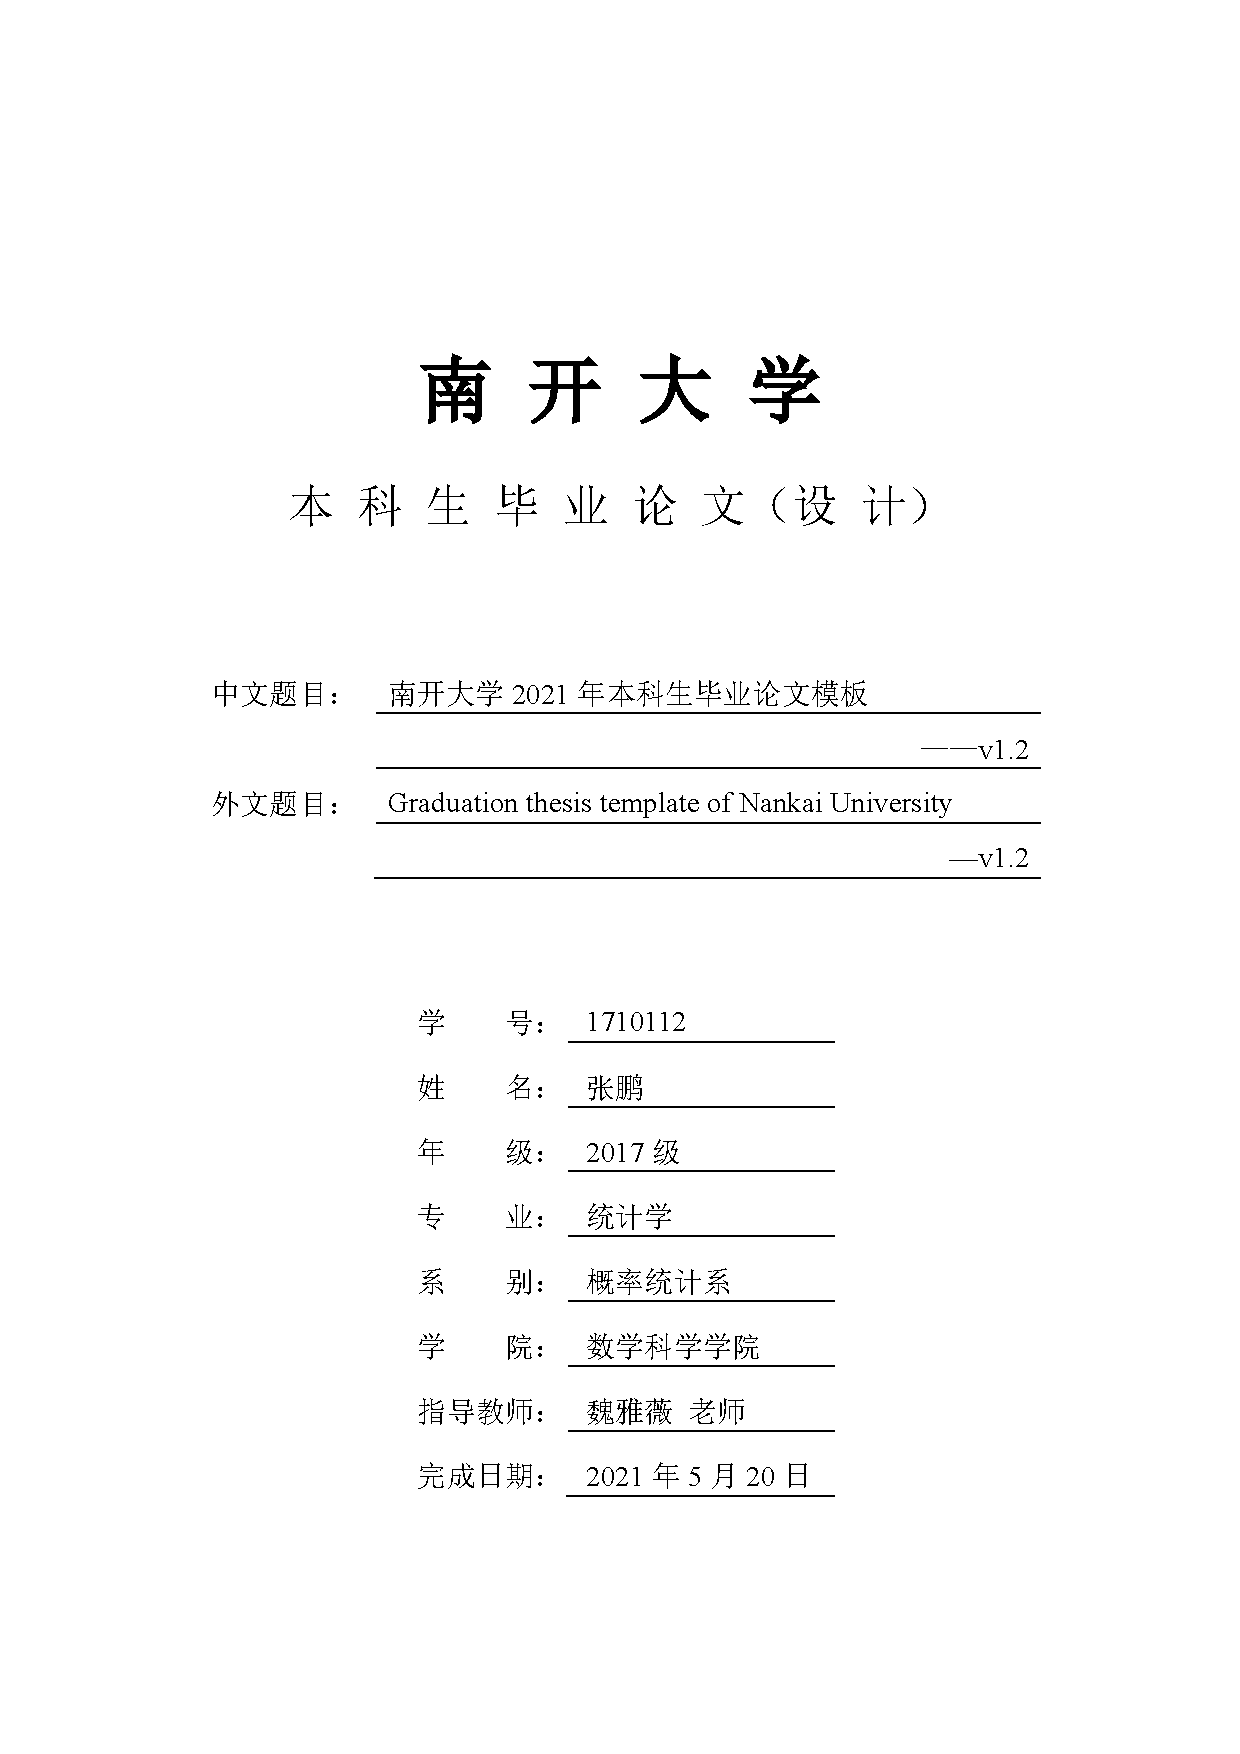
\includepdf[pages=1,pagecommand={},width=\textwidth,trim=28mm 25.4mm 28mm 25.4mm, clip]{cover/cover1.pdf} % 左 下 右 上
    
\includepdf[pages=1,pagecommand={},width=\textwidth,trim=28mm 25.4mm 28mm 25.4mm, clip]{cover/cover2.pdf}
    \pagenumbering{arabic}
}


\newenvironment{NKUAbstractZh} % 中文摘要
{
    \renewcommand{\abstractname}{\zihao{4} 摘\quad 要}
    \pagenumbering{Roman}
    \begin{abstract}\zihao{-4}
}
{
    \end{abstract}
    \newpage
}

\newenvironment{NKUAbstractEn} % 英文摘要
{
    \renewcommand{\abstractname}{\zihao{4} Abstract}
    \begin{abstract}\zihao{-4}
}
{
    \end{abstract}
    \newpage
}

\newcommand{\NKUAppendixSection}{ % 附录节
    \clearpage
    % 写法一:默认的 \appendix 命令
    %\appendix % 该行以后的章节都无编号
    %\ctexset{section/aftername = \hspace{6pt}} % 恢复间距
    %
    % 写法二:由于NK应该是只需要一个目录,因此采用了下面的方法
    \setcounter{secnumdepth}{0} % 抑制section的编号
    \section{\texorpdfstring{附\quad 录}{附录}} % 正常情况下应该是\section{附\quad 录},但为了兼容PDF书签功能这么写
}


\newcommand{\NKUThanksSection}{ % 致谢节
   \clearpage
    \section{\texorpdfstring{致\quad 谢}{致谢}} % 正常情况下应该是\section{致\quad 谢},但为了兼容PDF书签功能这么写
}
